\chapter{\RU{Шутка с игрой Color Lines}\EN{Color Lines game practical joke}}
\label{chap:color_lines}

\RU{Это очень популярная игра с большим количеством реализаций}\EN{This is a very popular game with several 
implementations exist}.
\RU{Я взял одну из них, с названием}\EN{I took one of them, called} BallTriX, \RU{от}\EN{from} 1997, 
\RU{доступную бесплатно на}\EN{available freely at} 
\url{http://www.download-central.ws/Win32/Games/B/BallTriX/}.
\RU{Вот как она выглядит}\EN{Here is how it looks}: \figref{fig:lines_1}.

\index{\CStandardLibrary!rand()}
\RU{Посмотрим, сможем ли мы найти генератор псевдослучайных чисел и и сделать с ним одну шутку.}
\EN{So let's see, will it be possible find random generator and do some trick with it.}
\IDA \RU{быстро распознает стандартную ф-цию}\EN{quickly recognize standard} \TT{\_rand} \RU{в}\EN{function in} 
\TT{balltrix.exe} \RU{по адресу}\EN{at} \TT{0x00403DA0}.
\IDA \RU{также показывает, что она вызывается только из одного места}\EN{also shows that it is called 
only from one place}:

\lstinputlisting{examples/lines/random.lst}

\RU{Я назову её}\EN{I'll call it} ``random''.
\RU{Пока не будем концентрироваться на самом коде ф-ции}\EN{Let's not to dive into this function's code yet}.

\RU{Эта ф-ция вызывается из трех мест}\EN{This function is reffered from 3 places}.

\RU{Вот первые два}\EN{Here is first two}:

\lstinputlisting{examples/lines/1.lst}

\EN{Here is the third}\RU{Вот третье}:

\lstinputlisting{examples/lines/2.lst}

\RU{Так что у ф-ции только один аргумент}\EN{So the function have only one argument}.
\RU{10 передается в первых двух случаях и 5 в третьем.}
\EN{10 is passed in first two cases and 5 in third.}
\RU{Мы также можем заметить что размер доски 10*10 и здесь 5 возможных цветов}\EN{We may also notice 
that the board has size 10*10 and there are 5 possible colors}.
\RU{Это оно}\EN{This is it}!
\RU{Стандартная ф-ция}\EN{The standard} \TT{rand()} \RU{возвращает число в пределах}\EN{function returns 
a number in} \TT{0..0x7FFF} \RU{и это неудобно, так что многие программисты пишут свою ф-цию,
возвращающую случайное число в некоторых заданных пределах}\EN{range and this is often inconvenient,
so many programmers implement their own random functions which returns a random number in specified range}.
\RU{В нашем случае, предел это}\EN{In our case, range is} $0..n-1$ \AndENRU $n$ \RU{передается как
единственный аргумент в ф-цию}\EN{is passed as the sole argument to the function}.
\RU{Мы можем быстро проверить это в отладчике}\EN{We can quickly check this in any debugger}.

\RU{Сделаем так, чтобы третий вызов ф-ции всегда возвращал ноль}\EN{So let's fix third function return at zero}.
\RU{Я в начале заменил три инструкции}\EN{I first replaced three instructions} (\TT{PUSH/CALL/ADD}) 
\RU{на}\EN{by} \ac{NOP}s.
\RU{Затем я добавил инструкцию}\EN{Then I add} \TT{XOR EAX, EAX}\RU{, для очистки регистра \EAX}\EN{ instruction, 
to clear \EAX register}.

\lstinputlisting{examples/lines/fixed.lst}

\RU{Что я сделал, это заменил вызов ф-ции}\EN{So what I did is replaced call to} \TT{random()} 
\RU{на код, всегда возвращающий ноль}\EN{function by a code which always returns zero}.

\RU{Теперь запустим}\EN{Let's run it now}: \figref{fig:lines_2}.
\RU{О да, это работает}\EN{Oh yes, it works}\footnote{\RU{Я однажды сделал это как 
шутку для моих сотрудников, в надежде что они перестанут играть. 
Надежды не оправдались.}\EN{I once did this as a joke for my coworkers with 
a hope they stop playing. They didn't.}}.

\RU{Но почему аргументы ф-ции}\EN{But why arguments to the} \TT{random()} \RU{это глобальные 
переменные}\EN{functions are global variables}?
\RU{Это просто потому что в настройках игры можно изменять размер доски, так что эти параметры не 
фиксированы}\EN{That's just because it's possible to change board size in game settings, 
so these values are not hardcoded}.
10 \AndENRU 5 \RU{это просто значения по умолчанию}\EN{values are just defaults}.

\begin{figure}[H]
\centering
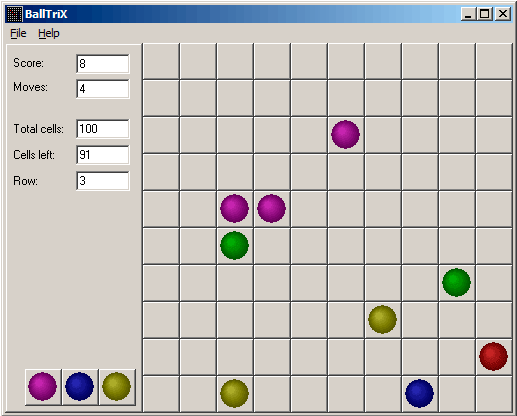
\includegraphics[scale=\FigScale]{examples/lines/1.png}
\caption{\RU{Обычный вид игры}\EN{How this game looks usually}}
\label{fig:lines_1}
\end{figure}

\begin{figure}[H]
\centering
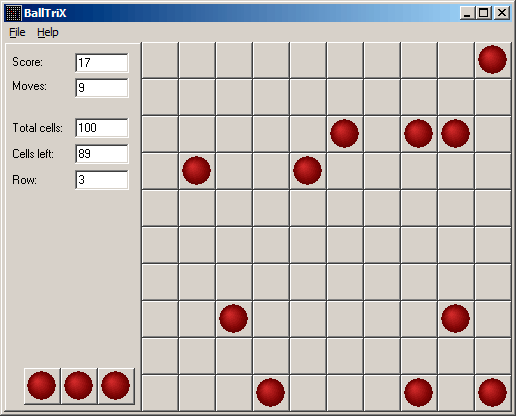
\includegraphics[scale=\FigScale]{examples/lines/2.png}
\caption{\RU{Шутка сработала}\EN{Practical joke works}}
\label{fig:lines_2}
\end{figure}
